Prior to analyzing the system as a whole, several analyses are performed on
various subsystems in order to examine important design trades at the subsystem
level and determine reasonable values for top-level design inputs.
Structural analysis is performed on the tube as the pod travels both over land and under water.
In these analysis, material properties of steel area used for the tube and
material properties of concrete are used for the tube in order to illustrate trends.
Both phases are analyzed prior to running the full system using values of
design variables suggested from previous research with safety factors where
appropriate \cite{Chin}. Then, cost function optimizations are performed with
appropriate design variables to determine which input values minimize material cost.
These values will then be fed into the whole system model to perform trade
studies on top-level design variables. It is understood that the values
obtained by performing optimization on subsystems will likely not be optimal
when the whole system is analyzed; however, these values are useful for
illustrating physical trends and system trades. The ScipyOptimizer is used to
minimize the scalar cost function using the Sequential Least Squares Programming
(SLSQP) algorithm for gradient based optimization \cite{GrayBenchmarking2013,Scipy}.
First, travel of the pod over land is analyzed. In this case, the pod travels
within a tube that is suspended on pylons of a given height above the ground.
To perform this analysis, multiple simplifying assumptions must be made. The
tube is assumed to have thin walls relative to the tube radius and thus will be
modeled as a thin-walled pressure vessel. The tube is assumed to be horizontal
and the height of the pylons is assumed to be constant. This allows a section
of the tube between two pylons to be modeled as a hollow cylindrical beam with
simple supports at its ends. Each pylon is modeled as a beam fixed at the
ground with axial and transverse loads applied to its end. The structure is
designed according to beam bending equations with the sectional weight of the
beam modeled as a distributed load and the mass of the pod as a point load at
the beam’s center (the structure is analyzed with the pod at the center of the
beam since this produces the highest bending stress in the tube).  With these
assumptions, two extreme structural configurations can be imagined: one in
which the tube is thick but is supported by pylons that are spaced very far apart,
and another in which the tube is thin but must be supported by many closely spaced pylons.
A cost function is developed by adding the cost of the tube material and the
cost of the supporting pylons per unit length, with the thickness of the tube
and the distance between pylons as design variables as shown in the equation

\begin{equation}
	\label{eq:tube_pylon_cost}
	Cost/Length = \frac{Tube Cost}{kg}*m'_{pod} + \frac{Pylon Cost}{kg}\frac{m_{pylon}}{\Delta x_{pylon}}
\end{equation}

Where $m’$ is the mass per unit length of the tube. This model, however, is
incomplete because the pylons can be any arbitrary size. To fix this problem,
the pylons are sized according to the buckling condition for a fixed column.
Imposing the condition allows for the spacing of the pylons to be computed in
terms of pylon radius and tube thickness using the equation

\begin{equation}
	\label{eq:pylon_spacing}
	\Delta x_{pylons} = \frac{\frac{\pi ^{2}Er_{p}^{4}}{16h^{2}} - \frac{1}{2}m_{pod}g}{\frac{1}{2}m^{'}g}
\end{equation}

Using this relationship, the cost function is defined with the tube thickness
and pylon radius as design variables. The final step is to appropriately constrain the optimization.
The minimum radius of the pylon is computed based on the yield strength of the pylon material.
Likewise, the minimum thickness of the tube is calculated using the buckling
condition for vacuum cylinders given by the equation \cite{Buckling}

\begin{equation}
	\label{eq:pres_buckling}
	P_{crit} = \frac{\gamma E}{4 ( 1-\nu^{2}  )} ( \frac{t}{r} )^{3}
\end{equation}

\begin{figure}
	\centering
	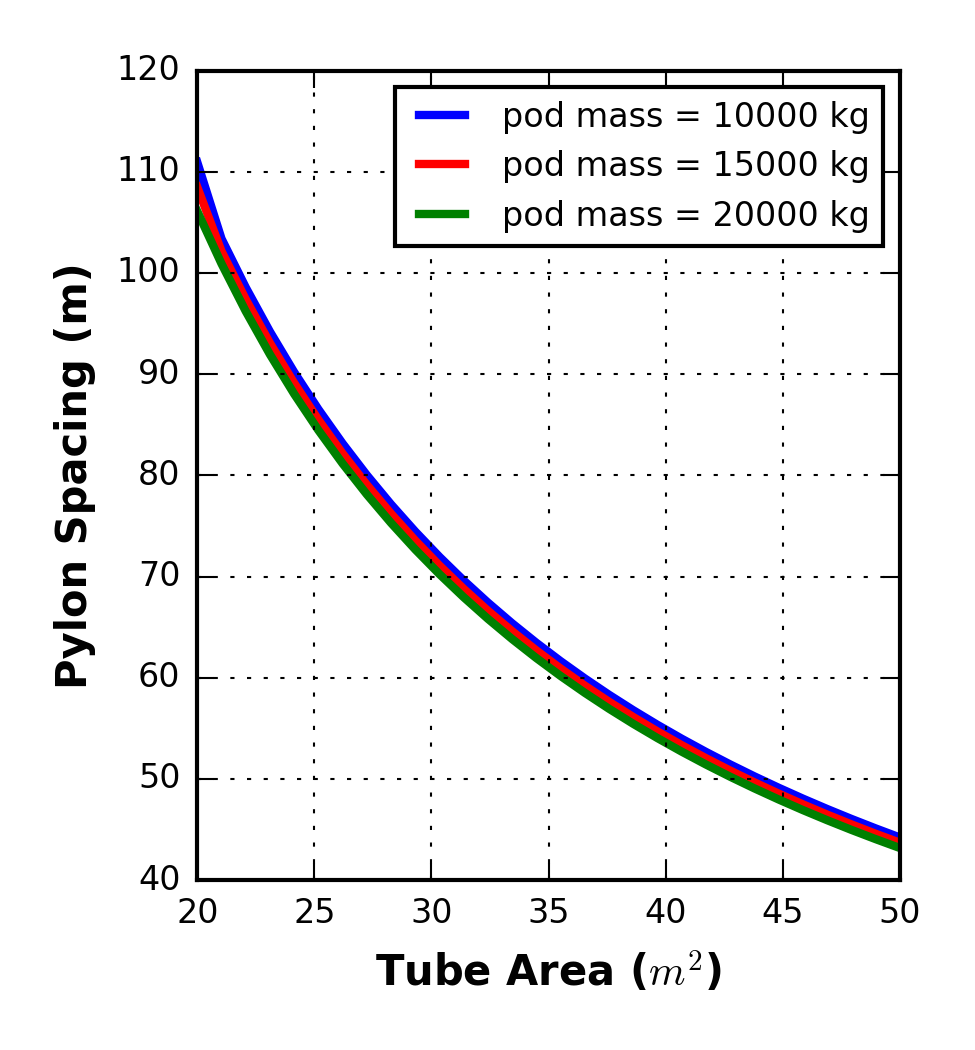
\includegraphics{../../images/graphs/overland_structural_trades/pylon_spacing_vs_tube_area.png}
	\caption{Optimal Pylon Spacing vs. Tube Area}
	\label{fig:pylon_spacing_vs_tube_area}
\end{figure}

For this analysis, the area of the tube is varied and the pylon spacing will is
recorded for different of pod masses. \Cref{fig:pylon_spacing_vs_tube_area}
shows that pylon spacing decreases significantly as tube area increases.
This is reasonable because, as tube area increases and becomes heavier, larger
pylons are needed to support the heavier load and a thicker tube is needed to
handle higher bending stress, both of which increase cost. This optimization
shows that moving the pylons closer together mitigates this cost penalty.
When performing analysis at the top level of the system, this plot along,
with the pylon buckling constraint, will be used to determine reasonable inputs
for tube thickness and pylon spacing for any given tube area or pod mass in
order to reflect optimal structural design conditions as closely as possible.
These results also give us preliminary insight into how favorably the Hyperloop
structure scales with pod capacity. For any given tube area I this regime,
increasing the pod mass from 10,000 kg to 20,000 kg results in a change in
pylon spacing of less than 2\%, with the sensitivity of pylon spacing to pod
mass decreasing for higher tube areas. This suggests that the mass of the tube
is dominant when sizing the structure of the system and that the pod mass is
negligible in this regime. This means that the capacity of each pod can be
increased with negligible ramifications on structural design. Pod capacity
trades will be discussed in greater detail in the following sections. However,
this analysis shows that pod capacity can be greatly scaled up with minimal
impact on structural design or the cost of materials and construction.
Structural analysis is also performed for underwater travel.
The model will have to be altered slightly from the model of the pod over land
in order to account for buoyancy. In this case, a section of the tube is
modeled as a hollow cylindrical beam subjected to a distributed load equal to
the difference between the sectional buoyancy and the sectional weight.
Travel underwater could have an interesting effect on structural design because
it is possible for the tube to be sized such that the entire weight of the
structure is suspended by its own buoyancy. In this case, support structure
would only be necessary to stabilize the structure against changing tides,
currents, and seismic activity rather than support the structural load.

\begin{figure}
	\centering
	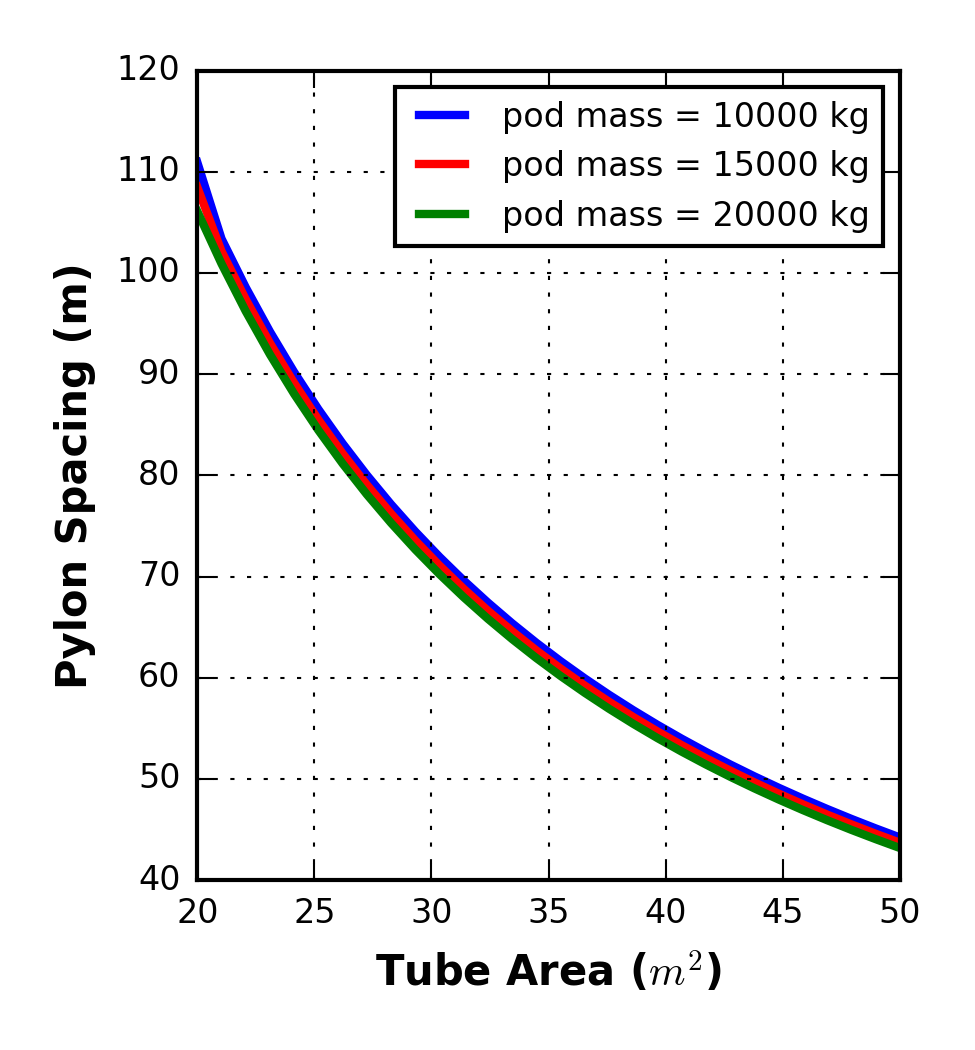
\includegraphics{../../images/graphs/overland_structural_trades/pylon_spacing_vs_tube_area.png}
	\caption{Thickness for Self-Suspension vs. Inner Area}
	\label{fig:thick_susp_vs_area}
\end{figure}

\Cref{fig:thick_susp_vs_area} shows the tube thickness at which the buoyant
force is equal to the weight of the tube allowing the tube structure to support itself.
Points above this curve will have weight greater than buoyancy and thus will
require pylons to support the weight. Likewise, points below this curve will
result in a buoyant force that is greater than the weight of the tube and would
require structures to anchor the tube at a certain depth.

\begin{figure}
	\centering
	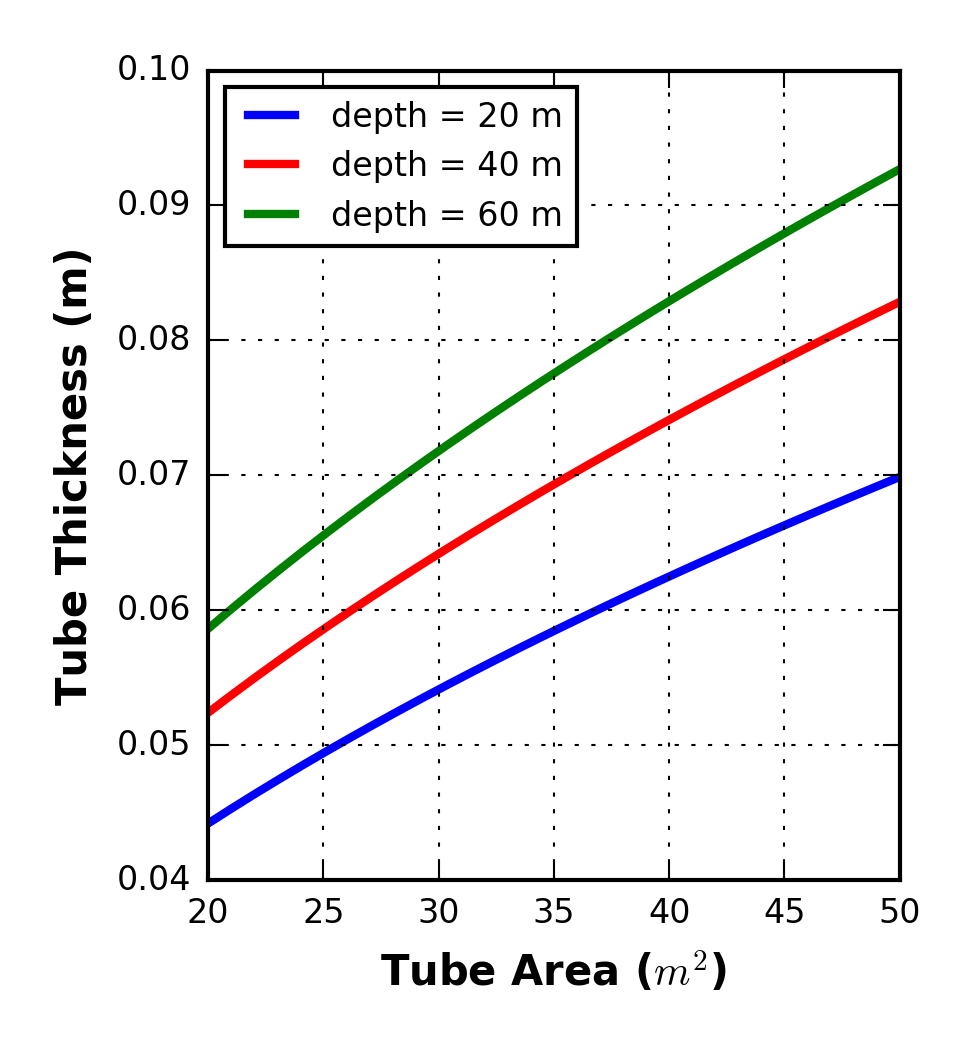
\includegraphics{../../images/graphs/underwater_structural_trades/tube_area_vs_depth.png}
	\caption{Tube Thickness vs. Tube Area of Travel Under Water}
	\label{fig:tube_thick_vs_tube_area_underwater}
\end{figure}

Traveling under water, unlike over land, allows the ambient pressure to change
significantly with the depth. \Cref{fig:tube_thick_vs_tube_area_underwater}
shows the sensitivity tube thickness to tube area for multiple different values of depth.
For large depths, thickness increases with tube area at a faster rate, which
results in increased material cost. It is important to note that the thickness
values calculated in this analysis are significantly below the values necessary
for self-suspension given in \cref{fig:thick_susp_vs_area}. Thus, for
underwater phases, it can be concluded that the Hyperloop structure would
likely be subjected to a buoyant force greater than the weight of the system
and would need to be designed in such a way that the pod is anchored to the sea
floor and stabilized in the event of disturbances.
The structural trade studies shown here suggest that there could be significant
benefits to traveling underwater as opposed to over land. The depth could be
chosen such that the tube could be thinner. Furthermore, it will likely be
easier to make the a straighter path traveling underwater because there will be
less buildings and features to contend with. Since the tube needs to be
air-tight regardless of whether travel is underwater or overland, either phase
will likely require the same level of manufacturing cost. While evaluating the
exact cost differential is beyond the scope of this paper due to the subjective
and volatile nature of capital cost evaluation, this system model suggests that
there could be real benefits from traveling underwater and should be the subject of further research.
